\section{LUẬT KẾT HỢP}

\subsection{Khái niệm}
Là một kỹ thuật cốt lõi trong khai phá dữ liệu dùng để phát hiện các mối quan hệ tiềm ẩn hoặc quy luật xuất hiện đồng thời giữa các đối tượng/mục dữ liệu trong một cơ sở dữ liệu lớn.\\
Dạng luật:
$$ X \rightarrow Y $$
Trong đó:
\begin{itemize}
    \item $X$ là tập hợp các mục dữ liệu điều kiện.
    \item $Y$ là tập hợp các mục dữ liệu được dự đoán sẽ xuất hiện cùng với $X$.
    \item $X \cap Y = \emptyset$ (không có phần tử chung).
\end{itemize}
Độ hỗ trợ và độ tin cậy của luật được tính như sau:
\[
\operatorname{support}(X\rightarrow Y)
=\operatorname{support}(X\cup Y),\qquad
\operatorname{confidence}(X\rightarrow Y)
=\frac{\operatorname{support}(X\cup Y)}{\operatorname{support}(X)}.
\]

\subsection{Ứng dụng}
Phân tích giỏ hàng siêu thị, thiết kế catalog, hệ thống gợi ý, phân tích dữ liệu sinh học.

\subsection{Thuật toán APRIORI}
\subsubsection{Ý tưởng}
Apriori khai phá các tập mục phổ biến theo từng kích thước: $1$-itemset, $2$-itemset, rồi các kích thước lớn hơn. Thuật toán dựa trên tính chất Apriori:"Nếu một tập mục là phổ biến thì mọi tập con khác rỗng của nó cũng phải phổ biến". Vì vậy, nếu một tập mục không đạt ngưỡng hỗ trợ, mọi tập lớn hơn chứa tập mục đó có thể bị loại mà không cần đếm.

\subsubsection{Ví dụ minh họa: tìm các tập mục phổ biến}
\textbf{Mô tả bài toán:} Một cửa hàng muốn tìm các mặt hàng thường được mua cùng nhau để hỗ trợ sắp xếp sản phẩm và đề xuất mua kèm. Tìm các tập mục phổ biến với ngưỡng hỗ trợ tối thiểu $\text{minsup}=2$ giao dịch (tương đương $2/5=40\%$).

\textbf{Mô tả dữ liệu:} Xét 5 giao dịch sau:
\begin{table}[H]
    \centering
    \begin{tabular}{|c|l|}
        \hline
        \textbf{Giao dịch} & \textbf{Các mặt hàng} \\
        \hline
        $T_1$ & $\{A,B,E\}$ \\ \hline
        $T_2$ & $\{B,D\}$ \\ \hline
        $T_3$ & $\{B,C\}$ \\ \hline
        $T_4$ & $\{A,B,D\}$ \\ \hline
        $T_5$ & $\{A,C\}$ \\ \hline
    \end{tabular}
    \caption{Giao dịch minh họa dùng chung cho Apriori và FP-Growth}
    \label{tab:association-example}
\end{table}

\textbf{Bước 1 - Đếm và lọc 1-itemset:} Đếm số giao dịch chứa từng mặt hàng:
\begin{center}
\begin{tabular}{|c|c|c|}
    \hline
    \textbf{Mặt hàng} & \textbf{Số lần xuất hiện} & \textbf{Kết quả} \\
    \hline
    $A$ & 3 & Phổ biến \\ \hline
    $B$ & 4 & Phổ biến \\ \hline
    $C$ & 2 & Phổ biến \\ \hline
    $D$ & 2 & Phổ biến \\ \hline
    $E$ & 1 & Loại \\
    \hline
\end{tabular}
\end{center}
Do đó $L_1=\{\{A\},\{B\},\{C\},\{D\}\}$; mặt hàng $E$ bị loại vì support nhỏ hơn 2.

\textbf{Bước 2 -- Sinh và đếm ứng viên 2-itemset:} Từ $L_1$, sinh các cặp rồi đếm số giao dịch chứa từng cặp:
\begin{center}
\begin{tabular}{|c|c|c|}
    \hline
    \textbf{Ứng viên} & \textbf{Support count} & \textbf{Kết quả} \\
    \hline
    $\{A,B\}$ & 2 & Phổ biến \\ \hline
    $\{A,C\}$ & 1 & Loại \\ \hline
    $\{A,D\}$ & 1 & Loại \\ \hline
    $\{B,C\}$ & 1 & Loại \\ \hline
    $\{B,D\}$ & 2 & Phổ biến \\ \hline
    $\{C,D\}$ & 0 & Loại \\
    \hline
\end{tabular}
\end{center}
Vậy $L_2=\{\{A,B\},\{B,D\}\}$.

\textbf{Bước 3 - Xét 3-itemset:} Hai tập trong $L_2$ không tạo được ứng viên 3-itemset theo phép nối Apriori. Hơn nữa, tập $\{A,B,D\}$ không thể phổ biến vì tập con $\{A,D\}$ không phổ biến. Do không còn ứng viên hợp lệ, thuật toán dừng. Các tập mục phổ biến là $L_1\cup L_2$.

\textbf{Bước 4 - Sinh luật kết hợp:} Nếu đặt $\text{minconf}=70\%$, luật $D\rightarrow B$ có:
\[
\operatorname{support}(D\rightarrow B)=\frac{2}{5}=40\%,\qquad
\operatorname{confidence}(D\rightarrow B)
=\frac{\operatorname{support}(\{B,D\})}{\operatorname{support}(\{D\})}
=\frac{2}{2}=100\%.
\]
Vì độ tin cậy đạt ngưỡng nên luật $D\rightarrow B$ được chấp nhận.

\subsubsection{Ưu điểm và nhược điểm}
\begin{itemize}
    \item \textbf{Ưu điểm:} Cách thực hiện tuần tự, dễ hiểu và dễ cài đặt; tính chất Apriori giúp loại bỏ nhiều ứng viên trước khi đếm.
    \item \textbf{Nhược điểm:} Cần quét cơ sở dữ liệu nhiều lần; khi có nhiều mặt hàng phổ biến, số lượng ứng viên có thể tăng nhanh và tốn thời gian/bộ nhớ.
\end{itemize}

\subsection{Thuật toán FP-GROWTH}
\subsubsection{Ý tưởng}
FP-Growth (Frequent Pattern Growth) khai phá tập mục phổ biến mà không tạo danh sách ứng viên như Apriori. Thuật toán thường quét cơ sở dữ liệu hai lần: lần đầu đếm support để xác định thứ tự mục; lần sau lọc, sắp thứ tự giao dịch và xây cây FP-Tree. Sau đó, thuật toán lần lượt khai phá cơ sở mẫu điều kiện (conditional pattern base) và cây điều kiện (conditional FP-Tree).

\subsubsection{Ví dụ minh họa: khai phá bằng FP-Tree}
Sử dụng lại bài toán, dữ liệu và ngưỡng $\text{minsup}=2$ ở phần Apriori.

\textbf{Bước 1 - Đếm support và sắp thứ tự mục:} Support đếm được là $B:4$, $A:3$, $C:2$, $D:2$, $E:1$. Loại $E$ vì không đạt minsup; sắp các mục còn lại theo support giảm dần, nếu bằng nhau thì theo thứ tự chữ cái: $B>A>C>D$.

\textbf{Bước 2 - Sắp xếp giao dịch và xây FP-Tree:} Loại mục không phổ biến, sau đó sắp các mục trong mỗi giao dịch theo thứ tự trên:
\begin{center}
\begin{tabular}{|c|c|}
    \hline
    \textbf{Giao dịch} & \textbf{Sau khi lọc và sắp xếp} \\
    \hline
    $T_1$ & $B\rightarrow A$ \\ \hline
    $T_2$ & $B\rightarrow D$ \\ \hline
    $T_3$ & $B\rightarrow C$ \\ \hline
    $T_4$ & $B\rightarrow A\rightarrow D$ \\ \hline
    $T_5$ & $A\rightarrow C$ \\
    \hline
\end{tabular}
\end{center}
Chèn lần lượt các đường giao dịch vào cây, gộp các tiền tố chung và cộng số đếm tại các nút:
\begin{figure}[H]
    \centering
    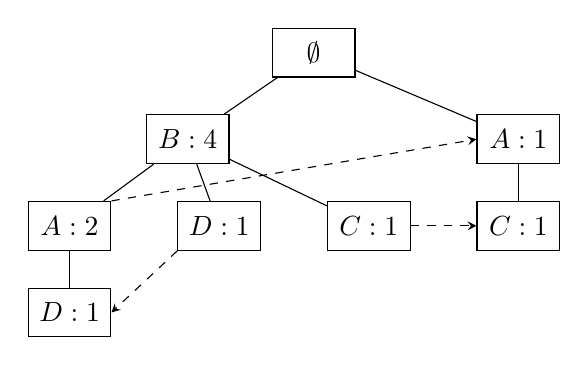
\begin{tikzpicture}[
        fpnode/.style={draw, rectangle, minimum width=1.05cm, minimum height=0.62cm, align=center},
        treeedge/.style={draw},
        nodelink/.style={draw, dashed, ->, >=stealth}
    ]
        \node[fpnode] (root) at (0,0) {$\emptyset$};
        \node[fpnode] (b) at (-1.6,-1.1) {$B:4$};
        \node[fpnode] (a-root) at (2.6,-1.1) {$A:1$};
        \node[fpnode] (a-b) at (-3.1,-2.2) {$A:2$};
        \node[fpnode] (d-b) at (-1.2,-2.2) {$D:1$};
        \node[fpnode] (c-b) at (0.7,-2.2) {$C:1$};
        \node[fpnode] (c-a) at (2.6,-2.2) {$C:1$};
        \node[fpnode] (d-ba) at (-3.1,-3.3) {$D:1$};

        \draw[treeedge] (root) -- (b);
        \draw[treeedge] (root) -- (a-root);
        \draw[treeedge] (b) -- (a-b);
        \draw[treeedge] (b) -- (d-b);
        \draw[treeedge] (b) -- (c-b);
        \draw[treeedge] (a-root) -- (c-a);
        \draw[treeedge] (a-b) -- (d-ba);

        \draw[nodelink] (a-b.north east) -- (a-root.west);
        \draw[nodelink] (c-b.east) -- (c-a.west);
        \draw[nodelink] (d-b.south west) -- (d-ba.east);
    \end{tikzpicture}
    \caption{FP-Tree của tập giao dịch minh họa}
    \label{fig:fp-tree-association-example}
\end{figure}
\noindent\textit{Đường liền biểu diễn nhánh cây; mũi tên nét đứt liên kết các nút cùng mặt hàng.}

\textbf{Bước 3 - Khai phá các mẫu điều kiện:} Xét các mục theo thứ tự support tăng dần:
\begin{itemize}
    \item \textbf{Mục $D$:} Các đường đi đến $D$ cho cơ sở mẫu điều kiện $\{\{B\}:1,\{B,A\}:1\}$. Trong đó $B$ có support 2, còn $A$ có support 1 nên chỉ giữ $B$. Suy ra tập phổ biến $\{B,D\}$ có support 2.
    \item \textbf{Mục $C$:} Cơ sở mẫu điều kiện là $\{\{B\}:1,\{A\}:1\}$. Không mục nào đạt support 2 trong cơ sở này, nên không tạo thêm tập phổ biến chứa $C$ ngoài $\{C\}$.
    \item \textbf{Mục $A$:} Đường đi có tiền tố đến $A$ là $\{B\}$ với số đếm 2; nút $A$ trực tiếp dưới gốc có tiền tố rỗng nên không tạo tổ hợp. Suy ra $\{A,B\}$ có support 2.
    \item \textbf{Mục $B$:} Không có tiền tố đứng trước $B$; support của $\{B\}$ là 4.
\end{itemize}

\textbf{Kết quả:} FP-Growth tìm được các tập phổ biến $\{A\}:3$, $\{B\}:4$, $\{C\}:2$, $\{D\}:2$, $\{A,B\}:2$ và $\{B,D\}:2$, trùng với kết quả Apriori. Từ đó cũng thu được luật $D\rightarrow B$ có support $40\%$ và confidence $100\%$.

\subsubsection{Ưu điểm và nhược điểm}
\begin{itemize}
    \item Ưu điểm: Không sinh ứng viên; thường hiệu quả khi dữ liệu có nhiều tiền tố chung vì FP-Tree nén được các giao dịch. Cơ sở dữ liệu gốc thường chỉ cần quét hai lần.
    \item Nhược điểm: Cấu trúc FP-Tree và các bước tạo mẫu điều kiện khó cài đặt, khó giải thích hơn Apriori; cây có thể tốn bộ nhớ nếu dữ liệu ít tiền tố chung hoặc có nhiều mẫu phân nhánh.
\end{itemize}